% !TeX root = ../main.tex
\chapter{Introducci\'on}
\label{cap:introduccion}

\section{Introducci\'on}
\label{sec:intro-intro}

Las constelaciones de sat\'elites en \'orbita terrestre baja (LEO) crecieron de
forma acelerada en la \'ultima d\'ecada. Los sat\'elites de observaci\'on de la
Tierra y las redes de comunicaciones generan hoy vol\'umenes de datos que
superan lo que sus enlaces de bajada pueden entregar. A esta limitaci\'on de
capacidad se suma la de disponibilidad. Un sat\'elite LEO es observado por una estaci\'on
terrestre determinada durante unos pocos minutos por pasada, as\'i que el
enlace directo a tierra funciona durante una fracci\'on peque\~na de la
\'orbita y los datos se acumulan a bordo hasta la ventana siguiente.

Un sat\'elite en \'orbita geoestacionaria (GEO) resuelve las dos cosas a la
vez. Desde su \'orbita ve una porci\'on grande de la trayectoria del sat\'elite
LEO y mantiene a la vez visibilidad permanente con una estaci\'on terrestre
fija. Un enlace LEO--GEO permite entonces retransmitir los datos en el momento
en que se generan, sin esperar la pr\'oxima pasada sobre la estaci\'on. Esto
aumenta la disponibilidad del canal y reduce el tiempo entre la adquisici\'on
de un dato y su llegada a tierra. Los sistemas de retransmisi\'on
geoestacionarios en operaci\'on, como el EDRS europeo, se construyeron con ese
prop\'osito~\cite{esa_edrs}.

La tecnolog\'ia que sostiene hoy estos enlaces es la \'optica. Las
constelaciones LEO operan enlaces \'opticos inter-satelitales (OISL) en
producci\'on, no como demostraci\'on tecnol\'ogica. A comienzos de 2024 SpaceX
report\'o que la malla \'optica de Starlink transportaba unos \num{42}
petabytes (\si{\peta\byte}) diarios sobre m\'as de \num{9000} enlaces
\'opticos instalados~\cite{starlink2024}. La \emph{Space Development Agency}
(SDA), la agencia del Departamento de Defensa de los Estados Unidos a cargo de
su red militar de sat\'elites, lleva adelante su Transport Layer con varios
cientos de sat\'elites LEO a unos \SI{1000}{\kilo\metre}, con OISL como
transporte principal~\cite{sda_transport}. Los terminales de esta
constelaci\'on tienen que cumplir el \emph{SDA Optical Communication Terminal
Standard}~\cite{sda_oct}. La Agencia Espacial Europea trabaja en ESTOL
(\emph{ESA Specification for Terabit/sec Optical Links}), cuya interfaz
a\'erea incorpora los requisitos de ese mismo est\'andar~\cite{esa_estol}.

\section{Evoluci\'on y proyecci\'on de los enlaces \'opticos inter-satelitales}
\label{sec:intro-industria}

La \cref{fig:evolucion-isl} re\'une las demostraciones en vuelo de enlaces
\'opticos inter-satelitales entre 2001 y 2024.

\begin{figure}[H]
  \centering
  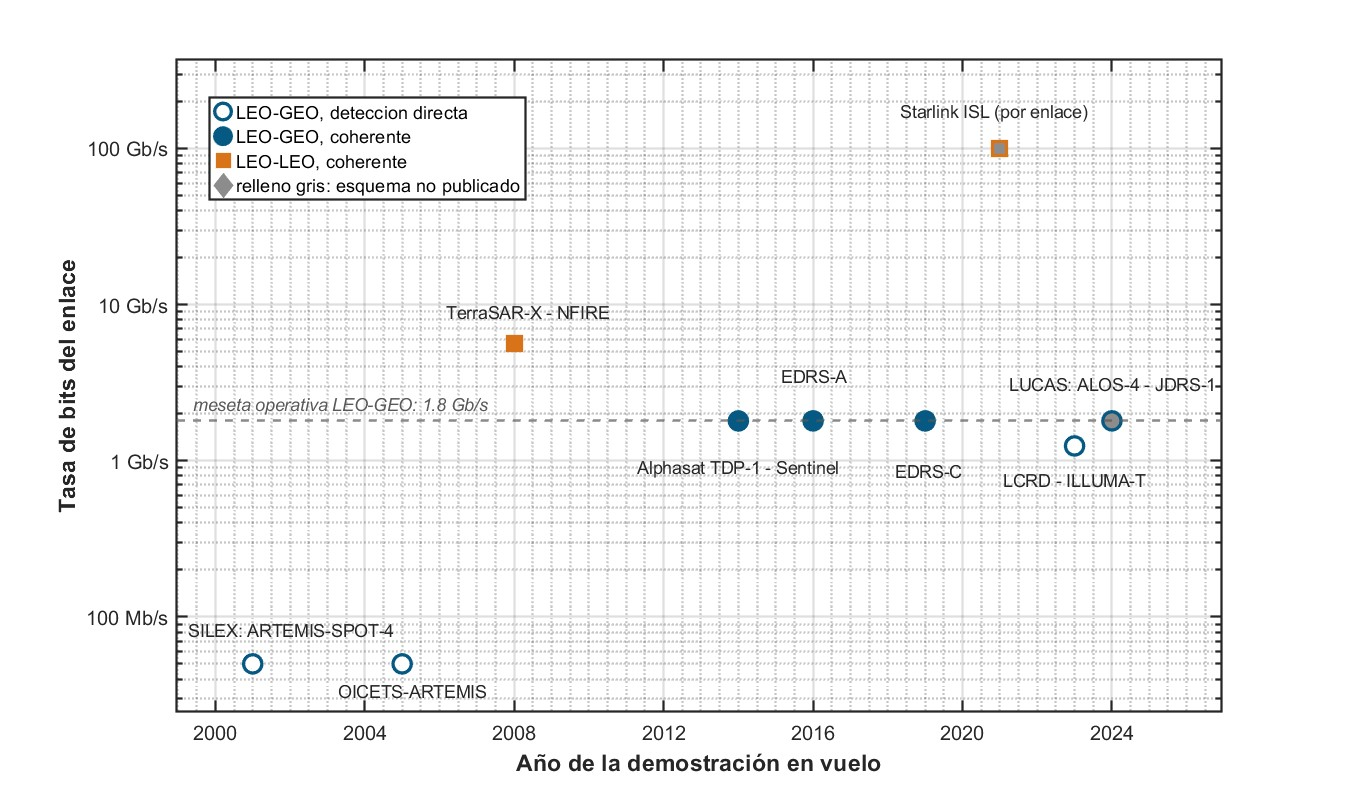
\includegraphics[width=\linewidth]{EvolucionTemporalEnlaceOptico}
  \caption[Evoluci\'on de los enlaces \'opticos inter-satelitales]{%
    Tasa de bits de los enlaces \'opticos inter-satelitales demostrados en
    vuelo. La forma del marcador indica el tipo de enlace (c\'irculo:
    LEO--GEO; cuadrado: LEO--LEO) y el relleno muestra el esquema de recepci\'on
    (hueco: sin oscilador local; lleno: coherente; gris: no publicado).
    Los enlaces LEO--GEO operativos permanecen en
    \SI{1.8}{\giga\bit\per\second} desde 2014, mientras las constelaciones
    comerciales LEO--LEO ya operan casi dos \'ordenes de magnitud por encima.
    Elaboraci\'on propia a partir de
    \cite{tolkernielsen2002,esa_silex2001,eoportal_artemis,esa_oicets2005,%
    smutny2009,tesat2018,esa_edrs,nasa_lcrd_illumat,nec_lucas2025,%
    chaudhry2021,starlink2024}.}
  \label{fig:evolucion-isl}
\end{figure}

En 2001 el experimento SILEX estableci\'o el primer enlace \'optico entre un
sat\'elite LEO y uno geoestacionario, entre SPOT-4 y ARTEMIS, a
\SI{50}{\mega\bit\per\second} con portadora en la banda de
\SIrange{800}{850}{\nano\metre} y fotodiodos de avalancha de
silicio~\cite{tolkernielsen2002,esa_silex2001}. El enlace entre OICETS/Kirari y
ARTEMIS, en 2005, repiti\'o exactamente la misma tasa en el sentido LEO hacia
GEO~\cite{eoportal_artemis,esa_oicets2005}. Cuatro a\~nos sin ganancia de
capacidad.

En 2008 los terminales LCT de Tesat enlazaron TerraSAR-X con NFIRE a
\SI{5.625}{\giga\bit\per\second} mediante recepci\'on homodina BPSK a
\SI{1064}{\nano\metre}~\cite{smutny2009,tesat2018}. Dos \'ordenes de magnitud
por encima de SILEX, sin un aumento del tama\~no de las \'opticas. Esta misma
familia de terminales es la que la Agencia Espacial Europea llev\'o a
operaci\'on en el sistema EDRS, primero como demostraci\'on entre Alphasat
TDP-1 y Sentinel-1A en 2014. Entr\'o en servicio con EDRS-A en 2016 y con
EDRS-C en 2019, siempre a \SI{1.8}{\giga\bit\per\second}~\cite{esa_edrs}.

En 2023 el par LCRD--ILLUMA-T cerr\'o el primer sistema de retransmisi\'on
\'optica bidireccional extremo a extremo de la NASA, entre la Estaci\'on
Espacial Internacional y un sat\'elite geoestacionario, a
\SI{1.2}{\giga\bit\per\second}~\cite{nasa_lcrd_illumat}. En 2024 el sistema
japon\'es LUCAS estableci\'o el enlace con DAICHI-4. En 2025 JAXA y NEC
reportaron la transmisi\'on de datos de misi\'on a
\SI{1.8}{\giga\bit\per\second} en banda de
\SI{1.5}{\micro\metre}~\cite{nec_lucas2025}. La presentaron como la
comunicaci\'on \'optica inter-satelital m\'as r\'apida del mundo, lo que fija
el estado del arte operativo en esa tasa. Diez a\~nos despu\'es de Alphasat, la
capacidad de un enlace LEO--GEO sigue siendo la misma.

El contraste con los enlaces LEO--LEO es grande. Starlink opera desde 2021 una
malla \'optica con capacidades del orden de \SI{100}{\giga\bit\per\second} por
enlace~\cite{chaudhry2021,starlink2024}, casi dos \'ordenes de magnitud por
encima del enlace de retransmisi\'on geoestacionario. La diferencia tiene dos
causas. En primer lugar se tiene el balance de potencia. Un enlace entre dos
sat\'elites LEO cubre unos pocos miles de kil\'ometros, mientras que un enlace
de retransmisi\'on geoestacionario cubre \SI{45000}{\kilo\metre}, lo que agrega
entre \num{19} y \SI{33}{\dB} de p\'erdida de espacio libre. Por otro lado
est\'a la forma en que se gestiona el programa. Un sistema de retransmisi\'on
GEO es un programa de interoperabilidad a quince a\~nos que congela una
generaci\'on de terminal, mientras que una constelaci\'on comercial renueva su
hardware cada pocos a\~nos.

La \cref{tab:capacidades} ordena estas capacidades por tecnolog\'ia de
transporte.

\begin{table}[htbp]
\centering
\begin{tabular}{llc}
\toprule
\textbf{Tecnolog\'ia} & \textbf{Fuente} & \textbf{Capacidad por enlace} \\
\midrule
Retransmisi\'on RF LEO--GEO, banda Ka         & \cite{nasa_katt}
                                     & $\sim$\SI{0.7}{\giga\bit\per\second} \\
Terminal \'optica comercial OOK-NRZ  & \cite{sda_oct,mynaric_condor}
                                     & \SIrange{0.31}{2.5}{\giga\bit\per\second} \\
Retransmisi\'on \'optica LEO--GEO en servicio & \cite{esa_edrs,nec_lucas2025}
                                     & \SI{1.8}{\giga\bit\per\second} \\
Malla \'optica LEO--LEO comercial    & \cite{starlink2024}
                                     & $\sim$\SI{100}{\giga\bit\per\second} \\
DP-QPSK coherente demostrado en tierra & \cite{scirep2022}
                                     & \SI{100}{\giga\bit\per\second} \\
\bottomrule
\end{tabular}
\caption[Capacidad por enlace seg\'un la tecnolog\'ia de transporte]{Capacidad
por enlace seg\'un la tecnolog\'ia de transporte. Valores representativos de
cada categor\'ia, no de cat\'alogo.}
\label{tab:capacidades}
\end{table}

De los enlaces inter-satelitales que operaron hasta hoy, todos los coherentes
pertenecen a la misma familia de terminales, con modulaci\'on binaria sobre una
\'unica polarizaci\'on. Hasta la fecha no se encontraron en la literatura
enlaces inter-satelitales operativos que empleen multiplexaci\'on en
polarizaci\'on. El est\'andar OCT de la SDA, que fija la interfaz de los
terminales comerciales actuales, especifica OOK-NRZ con un m\'aximo de
\SI{2.5}{\giga\bit\per\second}. Del transmisor no dice nada sobre
polarizaci\'on. Al receptor solo le pide que acepte cualquier estado de
polarizaci\'on recibido~\cite{sda_oct}. El formato de modulaci\'on que se
estudia en este trabajo ya se demostr\'o en enlaces \'opticos inal\'ambricos
terrestres. Por ejemplo, un enlace DP-QPSK de \SI{27.95}{\giga\baud} entre una
azotea y un dron, a velocidades angulares de seguimiento LEO, sostuvo
\SI{100}{\giga\bit\per\second}~\cite{scirep2022}.

Hasta la fecha, el incremento de la tasa de transmisi\'on en enlaces
satelitales apunt\'o a aumentar la tasa de s\'imbolo en modulaciones no
coherentes, combinado con la multiplexaci\'on en longitud de onda (WDM). Esta
es precisamente la direcci\'on que los programas en curso ya no pueden seguir.
Tanto el est\'andar OCT de la SDA como las especificaciones ESTOL de la ESA
apuntan a capacidades agregadas del orden del terabit por segundo. Subir solo
la tasa de s\'imbolo exigir\'ia anchos de banda y consumos incompatibles con
una plataforma LEO. Multiplexar en longitud de onda es el otro eje disponible.
El propio est\'andar OCT ya define \num{44} canales en banda
C~\cite{sda_oct}. Pero cada canal que se agrega conlleva sumar un l\'aser, un
amplificador y un terminal m\'as caro. El camino que queda es el que la
comunicaci\'on por fibra \'optica recorri\'o hace quince a\~nos. Pasar de
modulaci\'on binaria a formatos multinivel multiplexados en las dos
polarizaciones. La complejidad que eso agrega se absorbe en procesamiento
digital.

En este contexto, el trabajo desarrollado en este Proyecto Integrador aborda la
primera etapa del camino, con el estudio de un receptor \'optico coherente
DP-QPSK para un enlace LEO--GEO.

\section{Definici\'on del problema}
\label{sec:intro-problema}

Para pasar de \SI{10}{\giga\bit\per\second} a m\'as de
\SI{100}{\giga\bit\per\second} no alcanza con subir la potencia. Se necesita
multiplexar en polarizaci\'on y usar formatos de fase multinivel. Esto exige
detecci\'on coherente con procesamiento digital de la se\~nal recibida.

Hay tres motivos principales que sustentan la elecci\'on de un enlace \'optico
coherente para comunicaciones entre sat\'elites:

\begin{enumerate}
  \item \textbf{Espectro:} El espectro de RF est\'a saturado y requiere
        licencia, coordinaci\'on y control de interferencia. Las frecuencias
        \'opticas no est\'an sujetas a ese r\'egimen.
  \item \textbf{Directividad del haz:} A frecuencias \'opticas la divergencia
        del haz es del orden de los microradianes, lo que permite reducir la
        interferencia con otros sat\'elites y dificultar la intercepci\'on.
  \item \textbf{Masa y consumo:} Aperturas de cent\'imetros en lugar de metros.
        Por ejemplo, una antena de RF en banda Ka necesitar\'ia decenas de
        metros para el mismo balance de potencia, seg\'un la
        \cref{sec:canal-geometria}.
\end{enumerate}

La detecci\'on coherente con procesamiento digital es una tecnolog\'ia madura y
ampliamente desplegada en los enlaces de fibra \'optica terrestres. Un enlace inter-satelital LEO--GEO, en cambio, impone condiciones
que no aparecen en una fibra. Se tienen presentes un desplazamiento Doppler de
varios \si{\giga\hertz} que var\'ia durante el pase, una rotaci\'on continua
del estado de polarizaci\'on y una OSNR limitada por las enormes p\'erdidas de
potencia en el canal. Estas son las condiciones que el receptor tiene que
tolerar antes de poder garantizar la viabilidad del enlace. Por esto, la pregunta que este trabajo
se propone abordar es la siguiente.

\begin{quote}
\emph{\textquestiondown Puede un receptor coherente DP-QPSK de
\SI{128}{\giga\bit\per\second} estimar y compensar las degradaciones propias de
un enlace LEO--GEO, de forma que se obtenga una BER pre-FEC por
debajo del umbral que un c\'odigo de bloque de decisi\'on dura (HD) necesita para
cerrar el enlace?}
\end{quote}

\section{Objetivos, alcances y limitaciones}
\label{sec:intro-objetivos}

\subsection*{Objetivo general}

Desarrollar y validar, mediante simulaciones num\'ericas e implementaci\'on
experimental, un receptor \'optico coherente a tasas de hasta
\SI{128}{\giga\bit\per\second} que emplee modulaci\'on QPSK en doble
polarizaci\'on (DP-QPSK) para un enlace inter-satelital LEO--GEO, y evaluar su
desempe\~no frente a las degradaciones del canal espacial.

\subsection*{Objetivos espec\'ificos}

\begin{enumerate}
  \item Implementar modelos matem\'aticos de la cadena completa, con el
        transmisor, el canal satelital y el receptor coherente.
  \item Implementar los algoritmos de procesamiento digital necesarios en el
        receptor: ortogonalizaci\'on, recuperaci\'on de frecuencia y de reloj,
        ecualizaci\'on adaptativa MIMO y recuperaci\'on de fase.
  \item Desarrollar el balance de potencia y determinar la OSNR disponible en
        un enlace con p\'erdidas compatibles con las de un enlace LEO--GEO.
  \item Evaluar la tolerancia del receptor al Doppler, a la rotaci\'on del
        estado de polarizaci\'on y al ruido del l\'aser.
  \item Validar experimentalmente el procesamiento sobre capturas de laboratorio.
\end{enumerate}

\subsection*{Alcances y limitaciones}

Se modela un enlace \'optico coherente inter-satelital LEO--GEO de
aproximadamente \SI{45000}{\kilo\metre}, con transmisi\'on en la banda C
(\SIrange{1530}{1565}{\nano\metre}) y portadora en \SI{1550}{\nano\metre},
equivalente a \SI{193.4}{\tera\hertz}. La se\~nal es DP-QPSK, con
\SI{2}{\bit} por s\'imbolo en cada una de las dos polarizaciones. La tasa de
dise\~no es \SI{32}{\giga\baud}, y se evaluaron adem\'as
\SI{12.5}{\giga\baud} y \SI{25}{\giga\baud}.s

Quedan fuera del alcance la adquisici\'on y el seguimiento del haz (PAT), la
codificaci\'on FEC, de modo que se reporta BER pre-FEC contra el umbral HD-FEC
del \SI{7}{\percent} ($3{,}8\times10^{-3}$), y la retransmisi\'on, ya que se
modela solo el terminal receptor y no un retransmisor transparente.

\section{Organizaci\'on de la tesis}
\label{sec:intro-organizacion}

\begin{itemize}
  \item \Cref{cap:coherentes}: se presentan los fundamentos de la detecci\'on
        coherente y se fijan las m\'etricas del trabajo, es decir la relaci\'on
        entre la OSNR y la relaci\'on se\~nal a ruido por s\'imbolo, el EVM y
        la BER pre-FEC contra el umbral HD-FEC.

  \item \Cref{cap:canal}: se modela el canal LEO--GEO. Se calcula la p\'erdida
        del enlace a \SI{45000}{\kilo\metre}, el offset Doppler y su
        variaci\'on durante el pase, y la rotaci\'on del estado de
        polarizaci\'on.

  \item \Cref{cap:transceptor}: se modelan el transmisor y el receptor
        coherente, incluyendo los l\'aseres, el modulador, el front end y el
        ADC.

  \item \Cref{cap:dsp}: se describe la cadena de procesamiento digital bloque
        por bloque, profundizando en la recuperaci\'on de frecuencia, que es la
        que fija el l\'imite de captura del receptor.

  \item \Cref{cap:enlace}: se unen los tres anteriores en el balance de
        potencia. Se obtiene la OSNR disponible en el peor instante del pase y
        se la compara con la que necesita el receptor simulado para llegar al
        umbral HD-FEC.

  \item \Cref{cap:tolerancias}: se estudian los efectos de cada deterioro sobre
        el receptor, se identifica el mecanismo que fija su l\'imite y se
        contrasta ese l\'imite con el valor que impone el enlace.

  \item \Cref{cap:experimental}: se implementa la cadena en el laboratorio y se
        procesan capturas reales con el mismo DSP, para tres tasas de
        s\'imbolo.

  \item \Cref{cap:conclusiones}: se re\'unen las conclusiones, se resumen los
        aportes del trabajo y se propone la continuaci\'on.

\end{itemize}
